\documentclass{standalone}
\usepackage{tikz}
\usetikzlibrary{patterns, positioning}


\begin{document}
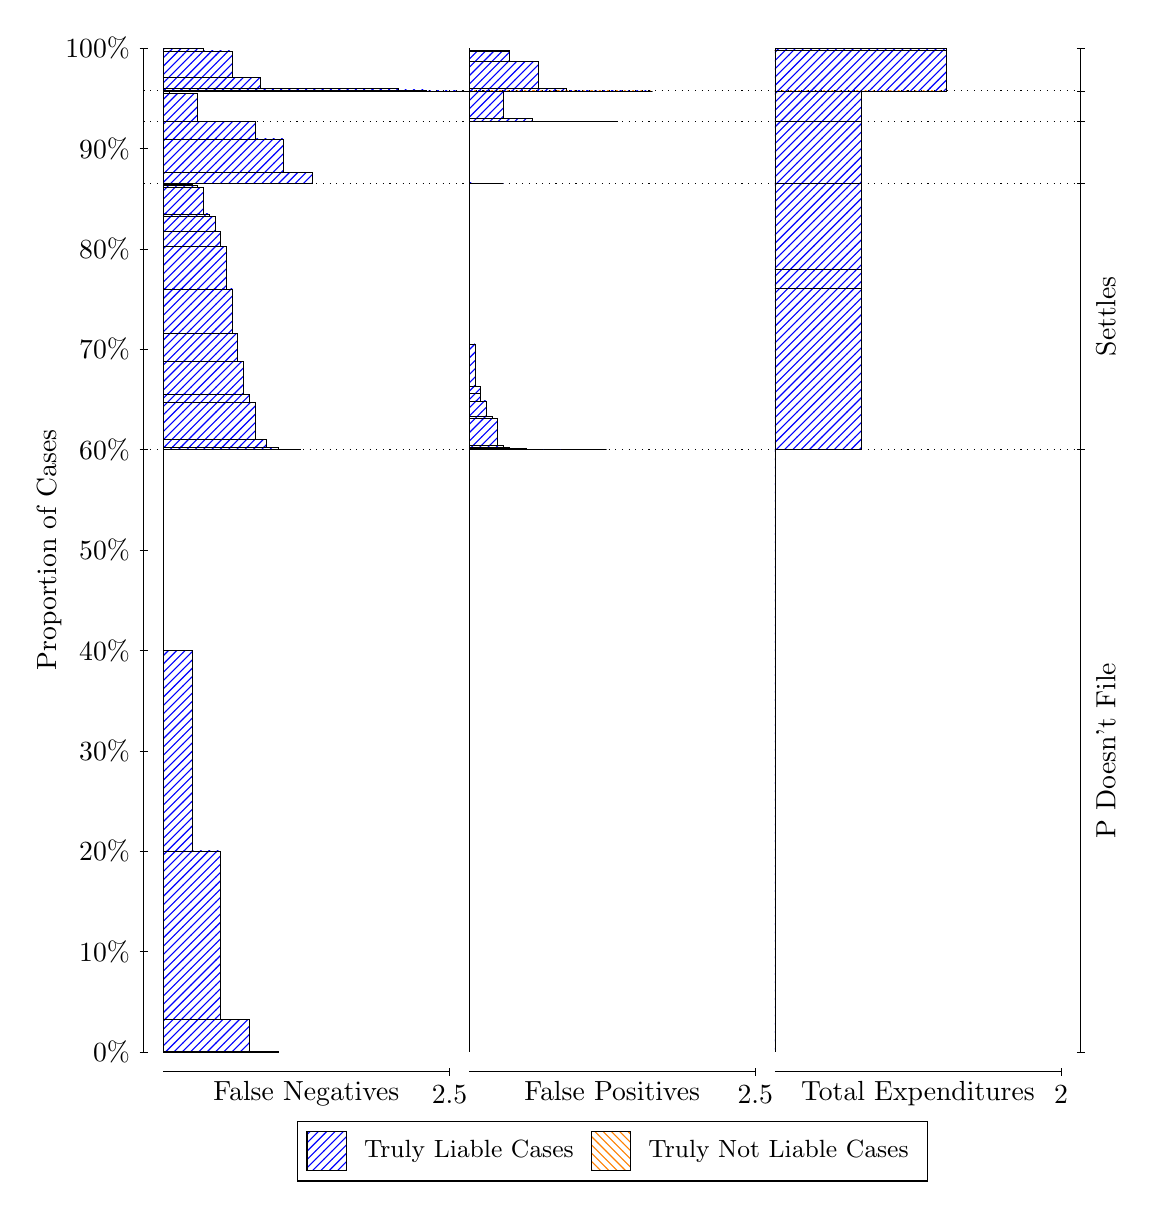
\begin{tikzpicture}
\draw[black, very thin] (1.5,1.75) -- (1.5,14.5);
\node[rotate=90, text=black, anchor=center] at (0.3, 8.125) {Proportion of Cases};
\draw[black, very thin] (1.45,1.75) -- (1.55,1.75);
\node[text=black, anchor=east] at (1.45, 1.75) {0\%};
\draw[black, very thin] (1.45,3.025) -- (1.55,3.025);
\node[text=black, anchor=east] at (1.45, 3.025) {10\%};
\draw[black, very thin] (1.45,4.3) -- (1.55,4.3);
\node[text=black, anchor=east] at (1.45, 4.3) {20\%};
\draw[black, very thin] (1.45,5.575) -- (1.55,5.575);
\node[text=black, anchor=east] at (1.45, 5.575) {30\%};
\draw[black, very thin] (1.45,6.85) -- (1.55,6.85);
\node[text=black, anchor=east] at (1.45, 6.85) {40\%};
\draw[black, very thin] (1.45,8.125) -- (1.55,8.125);
\node[text=black, anchor=east] at (1.45, 8.125) {50\%};
\draw[black, very thin] (1.45,9.4) -- (1.55,9.4);
\node[text=black, anchor=east] at (1.45, 9.4) {60\%};
\draw[black, very thin] (1.45,10.675) -- (1.55,10.675);
\node[text=black, anchor=east] at (1.45, 10.675) {70\%};
\draw[black, very thin] (1.45,11.95) -- (1.55,11.95);
\node[text=black, anchor=east] at (1.45, 11.95) {80\%};
\draw[black, very thin] (1.45,13.225) -- (1.55,13.225);
\node[text=black, anchor=east] at (1.45, 13.225) {90\%};
\draw[black, very thin] (1.45,14.5) -- (1.55,14.5);
\node[text=black, anchor=east] at (1.45, 14.5) {100\%};

\draw[black, very thin] (13.4,1.75) -- (13.4,14.5);
\draw[black, very thin] (13.35,1.75) -- (13.45,1.75);
\node[anchor=west] at (13.35, 1.75) {};
\draw[black, very thin] (13.35,9.4013) -- (13.45,9.4013);
\node[anchor=west] at (13.35, 9.4013) {};
\draw[black, very thin] (13.35,12.784) -- (13.45,12.784);
\node[anchor=west] at (13.35, 12.784) {};
\draw[black, very thin] (13.35,13.572) -- (13.45,13.572);
\node[anchor=west] at (13.35, 13.572) {};
\draw[black, very thin] (13.35,13.957) -- (13.45,13.957);
\node[anchor=west] at (13.35, 13.957) {};
\draw[black, very thin] (13.35,14.5) -- (13.45,14.5);
\node[anchor=west] at (13.35, 14.5) {};

\draw[black, very thin, pattern color=blue, pattern=north east lines] (1.75,1.75) rectangle (3.2033,1.7541);
\draw[black, very thin, pattern color=blue, pattern=north east lines] (1.75,1.7541) rectangle (2.84,2.1592);
\draw[black, very thin, pattern color=blue, pattern=north east lines] (1.75,2.1592) rectangle (2.4767,4.3047);
\draw[black, very thin, pattern color=blue, pattern=north east lines] (1.75,4.3047) rectangle (2.1133,6.8513);
\draw[black, very thin, pattern color=orange, pattern=north west lines] (1.75,6.8513) rectangle (1.75,6.8513);
\draw[black, very thin, pattern color=blue, pattern=north east lines] (1.75,6.8513) rectangle (1.75,9.4013);
\draw[black, very thin, pattern color=blue, pattern=north east lines] (1.75,9.4013) rectangle (3.494,9.4022);
\draw[black, very thin, pattern color=blue, pattern=north east lines] (1.75,9.4022) rectangle (3.3487,9.4032);
\draw[black, very thin, pattern color=blue, pattern=north east lines] (1.75,9.4032) rectangle (3.2033,9.4289);
\draw[black, very thin, pattern color=blue, pattern=north east lines] (1.75,9.4289) rectangle (3.1307,9.429);
\draw[black, very thin, pattern color=blue, pattern=north east lines] (1.75,9.429) rectangle (3.058,9.4333);
\draw[black, very thin, pattern color=blue, pattern=north east lines] (1.75,9.4333) rectangle (3.058,9.5259);
\draw[black, very thin, pattern color=blue, pattern=north east lines] (1.75,9.5259) rectangle (2.9853,9.5261);
\draw[black, very thin, pattern color=blue, pattern=north east lines] (1.75,9.5261) rectangle (2.9127,9.9983);
\draw[black, very thin, pattern color=blue, pattern=north east lines] (1.75,9.9983) rectangle (2.84,10.109);
\draw[black, very thin, pattern color=blue, pattern=north east lines] (1.75,10.109) rectangle (2.7673,10.519);
\draw[black, very thin, pattern color=blue, pattern=north east lines] (1.75,10.519) rectangle (2.6947,10.519);
\draw[black, very thin, pattern color=blue, pattern=north east lines] (1.75,10.519) rectangle (2.6947,10.879);
\draw[black, very thin, pattern color=blue, pattern=north east lines] (1.75,10.879) rectangle (2.622,11.442);
\draw[black, very thin, pattern color=blue, pattern=north east lines] (1.75,11.442) rectangle (2.622,11.442);
\draw[black, very thin, pattern color=blue, pattern=north east lines] (1.75,11.442) rectangle (2.5493,11.977);
\draw[black, very thin, pattern color=blue, pattern=north east lines] (1.75,11.977) rectangle (2.4767,12.168);
\draw[black, very thin, pattern color=blue, pattern=north east lines] (1.75,12.168) rectangle (2.404,12.36);
\draw[black, very thin, pattern color=blue, pattern=north east lines] (1.75,12.36) rectangle (2.404,12.36);
\draw[black, very thin, pattern color=blue, pattern=north east lines] (1.75,12.36) rectangle (2.3313,12.36);
\draw[black, very thin, pattern color=blue, pattern=north east lines] (1.75,12.36) rectangle (2.3313,12.393);
\draw[black, very thin, pattern color=blue, pattern=north east lines] (1.75,12.393) rectangle (2.3313,12.394);
\draw[black, very thin, pattern color=blue, pattern=north east lines] (1.75,12.394) rectangle (2.2587,12.729);
\draw[black, very thin, pattern color=blue, pattern=north east lines] (1.75,12.729) rectangle (2.2587,12.729);
\draw[black, very thin, pattern color=blue, pattern=north east lines] (1.75,12.729) rectangle (2.186,12.755);
\draw[black, very thin, pattern color=blue, pattern=north east lines] (1.75,12.755) rectangle (2.1133,12.768);
\draw[black, very thin, pattern color=blue, pattern=north east lines] (1.75,12.768) rectangle (2.0407,12.773);
\draw[black, very thin, pattern color=blue, pattern=north east lines] (1.75,12.773) rectangle (2.0407,12.773);
\draw[black, very thin, pattern color=blue, pattern=north east lines] (1.75,12.773) rectangle (1.968,12.773);
\draw[black, very thin, pattern color=blue, pattern=north east lines] (1.75,12.773) rectangle (1.968,12.773);
\draw[black, very thin, pattern color=blue, pattern=north east lines] (1.75,12.773) rectangle (1.968,12.773);
\draw[black, very thin, pattern color=blue, pattern=north east lines] (1.75,12.773) rectangle (1.8953,12.784);
\draw[black, very thin, pattern color=blue, pattern=north east lines] (1.75,12.784) rectangle (1.8953,12.784);
\draw[black, very thin, pattern color=blue, pattern=north east lines] (1.75,12.784) rectangle (1.8227,12.784);
\draw[black, very thin, pattern color=orange, pattern=north west lines] (1.75,12.784) rectangle (1.75,12.784);
\draw[black, very thin, pattern color=blue, pattern=north east lines] (1.75,12.784) rectangle (1.75,12.784);
\draw[black, very thin, pattern color=blue, pattern=north east lines] (1.75,12.784) rectangle (3.6393,12.918);
\draw[black, very thin, pattern color=blue, pattern=north east lines] (1.75,12.918) rectangle (3.276,13.345);
\draw[black, very thin, pattern color=blue, pattern=north east lines] (1.75,13.345) rectangle (2.9127,13.569);
\draw[black, very thin, pattern color=blue, pattern=north east lines] (1.75,13.569) rectangle (2.5493,13.572);
\draw[black, very thin, pattern color=blue, pattern=north east lines] (1.75,13.572) rectangle (2.186,13.572);
\draw[black, very thin, pattern color=orange, pattern=north west lines] (1.75,13.572) rectangle (1.75,13.572);
\draw[black, very thin, pattern color=blue, pattern=north east lines] (1.75,13.572) rectangle (2.186,13.924);
\draw[black, very thin, pattern color=blue, pattern=north east lines] (1.75,13.924) rectangle (1.8227,13.957);
\draw[black, very thin, pattern color=orange, pattern=north west lines] (1.75,13.957) rectangle (1.75,13.957);
\draw[black, very thin, pattern color=blue, pattern=north east lines] (1.75,13.957) rectangle (1.75,13.957);
\draw[black, very thin, pattern color=blue, pattern=north east lines] (1.75,13.957) rectangle (5.8193,13.957);
\draw[black, very thin, pattern color=blue, pattern=north east lines] (1.75,13.957) rectangle (5.456,13.957);
\draw[black, very thin, pattern color=blue, pattern=north east lines] (1.75,13.957) rectangle (5.0927,13.967);
\draw[black, very thin, pattern color=blue, pattern=north east lines] (1.75,13.967) rectangle (4.7293,13.985);
\draw[black, very thin, pattern color=blue, pattern=north east lines] (1.75,13.985) rectangle (4.366,13.985);
\draw[black, very thin, pattern color=blue, pattern=north east lines] (1.75,13.985) rectangle (4.0027,13.985);
\draw[black, very thin, pattern color=blue, pattern=north east lines] (1.75,13.985) rectangle (3.712,13.985);
\draw[black, very thin, pattern color=blue, pattern=north east lines] (1.75,13.985) rectangle (3.6393,13.985);
\draw[black, very thin, pattern color=blue, pattern=north east lines] (1.75,13.985) rectangle (3.3487,13.991);
\draw[black, very thin, pattern color=blue, pattern=north east lines] (1.75,13.991) rectangle (2.9853,14.128);
\draw[black, very thin, pattern color=blue, pattern=north east lines] (1.75,14.128) rectangle (2.622,14.465);
\draw[black, very thin, pattern color=blue, pattern=north east lines] (1.75,14.465) rectangle (2.2587,14.5);
\draw[black, very thin, pattern color=blue, pattern=north east lines] (1.75,14.5) rectangle (1.8953,14.5);
\draw[black, very thin, pattern color=orange, pattern=north west lines] (1.75,14.5) rectangle (1.75,14.5);
\draw[black, very thin, pattern color=blue, pattern=north east lines] (1.75,14.5) rectangle (1.75,14.5);
\draw[black, very thin, pattern color=orange, pattern=north west lines] (5.6333,1.75) rectangle (5.6333,1.75);
\draw[black, very thin, pattern color=blue, pattern=north east lines] (5.6333,1.75) rectangle (5.6333,9.4013);
\draw[black, very thin, pattern color=orange, pattern=north west lines] (5.6333,9.4013) rectangle (7.3773,9.4013);
\draw[black, very thin, pattern color=blue, pattern=north east lines] (5.6333,9.4013) rectangle (7.3773,9.4013);
\draw[black, very thin, pattern color=orange, pattern=north west lines] (5.6333,9.4013) rectangle (7.232,9.4013);
\draw[black, very thin, pattern color=blue, pattern=north east lines] (5.6333,9.4013) rectangle (7.232,9.4013);
\draw[black, very thin, pattern color=orange, pattern=north west lines] (5.6333,9.4013) rectangle (7.0867,9.4013);
\draw[black, very thin, pattern color=blue, pattern=north east lines] (5.6333,9.4013) rectangle (7.0867,9.4013);
\draw[black, very thin, pattern color=blue, pattern=north east lines] (5.6333,9.4013) rectangle (7.014,9.4013);
\draw[black, very thin, pattern color=orange, pattern=north west lines] (5.6333,9.4013) rectangle (6.9413,9.4013);
\draw[black, very thin, pattern color=blue, pattern=north east lines] (5.6333,9.4013) rectangle (6.9413,9.4013);
\draw[black, very thin, pattern color=blue, pattern=north east lines] (5.6333,9.4013) rectangle (6.8687,9.4013);
\draw[black, very thin, pattern color=orange, pattern=north west lines] (5.6333,9.4013) rectangle (6.796,9.4013);
\draw[black, very thin, pattern color=blue, pattern=north east lines] (5.6333,9.4013) rectangle (6.796,9.4013);
\draw[black, very thin, pattern color=blue, pattern=north east lines] (5.6333,9.4013) rectangle (6.7233,9.4013);
\draw[black, very thin, pattern color=orange, pattern=north west lines] (5.6333,9.4013) rectangle (6.6507,9.4013);
\draw[black, very thin, pattern color=blue, pattern=north east lines] (5.6333,9.4013) rectangle (6.6507,9.4013);
\draw[black, very thin, pattern color=blue, pattern=north east lines] (5.6333,9.4013) rectangle (6.578,9.4013);
\draw[black, very thin, pattern color=blue, pattern=north east lines] (5.6333,9.4013) rectangle (6.5053,9.4013);
\draw[black, very thin, pattern color=orange, pattern=north west lines] (5.6333,9.4013) rectangle (6.5053,9.4013);
\draw[black, very thin, pattern color=blue, pattern=north east lines] (5.6333,9.4013) rectangle (6.5053,9.4013);
\draw[black, very thin, pattern color=blue, pattern=north east lines] (5.6333,9.4013) rectangle (6.4327,9.4013);
\draw[black, very thin, pattern color=orange, pattern=north west lines] (5.6333,9.4013) rectangle (6.36,9.4013);
\draw[black, very thin, pattern color=blue, pattern=north east lines] (5.6333,9.4013) rectangle (6.36,9.4126);
\draw[black, very thin, pattern color=blue, pattern=north east lines] (5.6333,9.4126) rectangle (6.2873,9.4127);
\draw[black, very thin, pattern color=orange, pattern=north west lines] (5.6333,9.4127) rectangle (6.2147,9.4127);
\draw[black, very thin, pattern color=blue, pattern=north east lines] (5.6333,9.4127) rectangle (6.2147,9.4127);
\draw[black, very thin, pattern color=blue, pattern=north east lines] (5.6333,9.4127) rectangle (6.2147,9.4177);
\draw[black, very thin, pattern color=blue, pattern=north east lines] (5.6333,9.4177) rectangle (6.142,9.4298);
\draw[black, very thin, pattern color=blue, pattern=north east lines] (5.6333,9.4298) rectangle (6.142,9.43);
\draw[black, very thin, pattern color=blue, pattern=north east lines] (5.6333,9.43) rectangle (6.0693,9.4562);
\draw[black, very thin, pattern color=blue, pattern=north east lines] (5.6333,9.4562) rectangle (5.9967,9.7917);
\draw[black, very thin, pattern color=blue, pattern=north east lines] (5.6333,9.7917) rectangle (5.924,9.825);
\draw[black, very thin, pattern color=blue, pattern=north east lines] (5.6333,9.825) rectangle (5.8513,9.825);
\draw[black, very thin, pattern color=blue, pattern=north east lines] (5.6333,9.825) rectangle (5.8513,10.018);
\draw[black, very thin, pattern color=blue, pattern=north east lines] (5.6333,10.018) rectangle (5.7787,10.114);
\draw[black, very thin, pattern color=blue, pattern=north east lines] (5.6333,10.114) rectangle (5.7787,10.209);
\draw[black, very thin, pattern color=blue, pattern=north east lines] (5.6333,10.209) rectangle (5.706,10.743);
\draw[black, very thin, pattern color=blue, pattern=north east lines] (5.6333,10.743) rectangle (5.6333,12.784);
\draw[black, very thin, pattern color=orange, pattern=north west lines] (5.6333,12.784) rectangle (6.0693,12.784);
\draw[black, very thin, pattern color=blue, pattern=north east lines] (5.6333,12.784) rectangle (6.0693,12.784);
\draw[black, very thin, pattern color=blue, pattern=north east lines] (5.6333,12.784) rectangle (5.706,12.787);
\draw[black, very thin, pattern color=blue, pattern=north east lines] (5.6333,12.787) rectangle (5.6333,13.572);
\draw[black, very thin, pattern color=orange, pattern=north west lines] (5.6333,13.572) rectangle (7.5227,13.572);
\draw[black, very thin, pattern color=blue, pattern=north east lines] (5.6333,13.572) rectangle (7.5227,13.572);
\draw[black, very thin, pattern color=blue, pattern=north east lines] (5.6333,13.572) rectangle (7.1593,13.572);
\draw[black, very thin, pattern color=blue, pattern=north east lines] (5.6333,13.572) rectangle (6.796,13.572);
\draw[black, very thin, pattern color=blue, pattern=north east lines] (5.6333,13.572) rectangle (6.4327,13.604);
\draw[black, very thin, pattern color=blue, pattern=north east lines] (5.6333,13.604) rectangle (6.0693,13.957);
\draw[black, very thin, pattern color=orange, pattern=north west lines] (5.6333,13.957) rectangle (7.9587,13.957);
\draw[black, very thin, pattern color=blue, pattern=north east lines] (5.6333,13.957) rectangle (7.9587,13.957);
\draw[black, very thin, pattern color=orange, pattern=north west lines] (5.6333,13.957) rectangle (7.5953,13.957);
\draw[black, very thin, pattern color=blue, pattern=north east lines] (5.6333,13.957) rectangle (7.5953,13.957);
\draw[black, very thin, pattern color=orange, pattern=north west lines] (5.6333,13.957) rectangle (7.232,13.957);
\draw[black, very thin, pattern color=blue, pattern=north east lines] (5.6333,13.957) rectangle (7.232,13.957);
\draw[black, very thin, pattern color=blue, pattern=north east lines] (5.6333,13.957) rectangle (6.8687,13.992);
\draw[black, very thin, pattern color=orange, pattern=north west lines] (5.6333,13.992) rectangle (6.8687,13.992);
\draw[black, very thin, pattern color=blue, pattern=north east lines] (5.6333,13.992) rectangle (6.8687,13.992);
\draw[black, very thin, pattern color=blue, pattern=north east lines] (5.6333,13.992) rectangle (6.5053,14.328);
\draw[black, very thin, pattern color=blue, pattern=north east lines] (5.6333,14.328) rectangle (6.5053,14.328);
\draw[black, very thin, pattern color=blue, pattern=north east lines] (5.6333,14.328) rectangle (6.142,14.464);
\draw[black, very thin, pattern color=blue, pattern=north east lines] (5.6333,14.464) rectangle (6.142,14.466);
\draw[black, very thin, pattern color=blue, pattern=north east lines] (5.6333,14.466) rectangle (5.7787,14.471);
\draw[black, very thin, pattern color=blue, pattern=north east lines] (5.6333,14.471) rectangle (5.7787,14.471);
\draw[black, very thin, pattern color=orange, pattern=north west lines] (5.6333,14.471) rectangle (5.6333,14.471);
\draw[black, very thin, pattern color=blue, pattern=north east lines] (5.6333,14.471) rectangle (5.6333,14.5);
\draw[black, very thin, pattern color=orange, pattern=north west lines] (9.5167,1.75) rectangle (9.5167,1.75);
\draw[black, very thin, pattern color=blue, pattern=north east lines] (9.5167,1.75) rectangle (9.5167,9.4013);
\draw[black, very thin, pattern color=orange, pattern=north west lines] (9.5167,9.4013) rectangle (10.607,9.4013);
\draw[black, very thin, pattern color=blue, pattern=north east lines] (9.5167,9.4013) rectangle (10.607,11.452);
\draw[black, very thin, pattern color=orange, pattern=north west lines] (9.5167,11.452) rectangle (10.607,11.452);
\draw[black, very thin, pattern color=blue, pattern=north east lines] (9.5167,11.452) rectangle (10.607,11.691);
\draw[black, very thin, pattern color=orange, pattern=north west lines] (9.5167,11.691) rectangle (10.607,11.691);
\draw[black, very thin, pattern color=blue, pattern=north east lines] (9.5167,11.691) rectangle (10.607,12.784);
\draw[black, very thin, pattern color=orange, pattern=north west lines] (9.5167,12.784) rectangle (10.607,12.784);
\draw[black, very thin, pattern color=blue, pattern=north east lines] (9.5167,12.784) rectangle (10.607,13.572);
\draw[black, very thin, pattern color=orange, pattern=north west lines] (9.5167,13.572) rectangle (10.607,13.572);
\draw[black, very thin, pattern color=blue, pattern=north east lines] (9.5167,13.572) rectangle (10.607,13.957);
\draw[black, very thin, pattern color=orange, pattern=north west lines] (9.5167,13.957) rectangle (11.697,13.957);
\draw[black, very thin, pattern color=blue, pattern=north east lines] (9.5167,13.957) rectangle (11.697,14.469);
\draw[black, very thin, pattern color=orange, pattern=north west lines] (9.5167,14.469) rectangle (11.697,14.469);
\draw[black, very thin, pattern color=blue, pattern=north east lines] (9.5167,14.469) rectangle (11.697,14.471);
\draw[black, very thin, pattern color=orange, pattern=north west lines] (9.5167,14.471) rectangle (11.697,14.471);
\draw[black, very thin, pattern color=blue, pattern=north east lines] (9.5167,14.471) rectangle (11.697,14.5);
\draw[black, dotted] (1.5,9.4013) -- (13.4,9.4013);
\draw[black, dotted] (1.5,12.784) -- (13.4,12.784);
\draw[black, dotted] (1.5,13.572) -- (13.4,13.572);
\draw[black, dotted] (1.5,13.957) -- (13.4,13.957);
\draw[black, very thin] (1.75,1.5) -- (5.3833,1.5);
\node[text=black, anchor=north] at (3.5667, 1.5) {False Negatives};
\draw[black, very thin] (5.3833,1.45) -- (5.3833,1.55);
\node[text=black, anchor=north] at (5.3833, 1.45) {2.5};

\draw[black, very thin] (5.6333,1.5) -- (9.2667,1.5);
\node[text=black, anchor=north] at (7.45, 1.5) {False Positives};
\draw[black, very thin] (9.2667,1.45) -- (9.2667,1.55);
\node[text=black, anchor=north] at (9.2667, 1.45) {2.5};

\draw[black, very thin] (9.5167,1.5) -- (13.15,1.5);
\node[text=black, anchor=north] at (11.333, 1.5) {Total Expenditures};
\draw[black, very thin] (13.15,1.45) -- (13.15,1.55);
\node[text=black, anchor=north] at (13.15, 1.45) {2};

\node[text=black, centered, rotate=90] at (13.72, 5.5756) {P Doesn't File};
\node[text=black, centered, rotate=90] at (13.72, 11.093) {Settles};




\draw (7.449999999999999,1.5) node[draw=none] (baseCoordinate) {};
\begin{scope}[align=center]
        \matrix[scale=0.5, draw=black, below=0.5cm of baseCoordinate, nodes={draw}, column sep=0.1cm]{
            \node[rectangle, draw, minimum width=0.5cm, minimum height=0.5cm, pattern color=blue, pattern=north east lines] {}; &
            \node[draw=none, font=\small, text=black] (B) {Truly Liable Cases}; &
            \node[rectangle, draw, minimum width=0.5cm, minimum height=0.5cm, pattern color=orange, pattern=north west lines] {}; &
            \node[draw=none, font=\small, text=black] (B) {Truly Not Liable Cases}; \\
            };
\end{scope}

\end{tikzpicture}
\end{document}